% Created 2014-05-28 Wed 12:26
\documentclass[t]{beamer}
\usepackage[utf8]{inputenc}
\usepackage[T1]{fontenc}
\usepackage{fixltx2e}
\usepackage{graphicx}
\usepackage{longtable}
\usepackage{float}
\usepackage{wrapfig}
\usepackage{soul}
\usepackage{textcomp}
\usepackage{marvosym}
\usepackage{wasysym}
\usepackage{latexsym}
\usepackage{amssymb}
\usepackage{hyperref}
\tolerance=1000
\mode<beamer>{\usetheme{TUD}}
\usepackage{tikz}
\usetikzlibrary{positioning,chains,arrows,shadows,fadings,shapes,backgrounds,snakes,matrix,patterns,plotmarks,trees,mindmap}
\usepackage{pgfpages} 
\graphicspath{{./}{figs/}{figures/}{../logos/}{../cfigures/}{../RTS-2011/figs/}{}}
\newcommand{\floor}[1]{\left\lfloor{#1}\right\rfloor}
\newcommand{\setof}[1]{\left\{{#1}\right\}}
\newcommand{\set}[2]{\left\{{#1}\mid{#2}\right\}}
\newcommand{\ceiling}[1]{\left\lceil{#1}\right\rceil}
\newcommand{\red}[1]{\textcolor{red}{#1}}
\newcommand{\blue}[1]{\textcolor{blue}{#1}}
\providecommand{\alert}[1]{\textbf{#1}}

\title{PCP in RTEMS}
\author{Kuan-Hsun Chen}

\institute{LS 12, TU Dortmund}
\date{05,08,2015}
\hypersetup{
  pdfkeywords={},
  pdfsubject={},
  pdfcreator={Emacs Org-mode version 7.9.3f}}

\tikzset{
    task/.style={shade, shading=radial, rectangle,minimum height=.1cm,
        inner color=#1!20, outer color=#1!60!gray},
    task1/.style={task=yellow, minimum width=13mm},
    task2/.style={task=green, minimum width=13mm},
    task3/.style={task=red, minimum width=13mm},
    task4/.style={task=orange, minimum width=13mm},
    task5/.style={task=blue, minimum width=13mm},
    task6/.style={task=purple, minimum width=13mm},
    task7/.style={task=cyan, minimum width=13mm},
    task8/.style={task=pink, minimum width=13mm},
}

\tikzstyle{circleNode}=[circle,thick,draw=blue!75,fill=blue!20,minimum size=6mm]
\tikzstyle{niceFill}=[thick,draw=blue!75,fill=blue!20,minimum size=6mm]

\begin{document}

\maketitle

\begin{frame}
\frametitle{Outline}

\begin{itemize}

\item Drawback in PIP

\item Introduction of PCP

\item PCP implementation

\item Exercises

\end{itemize} % ends low level
\end{frame}

\begin{frame}
\frametitle{Drawback?}
Now we have PIP to mitigate the priority inversion and prevent the starvation of higher priority. However there is still a drawback:
\begin{itemize}
  \item PIP might cause a \emph{\textcolor{blue}{deadlock}} if there are
  multiple resources

    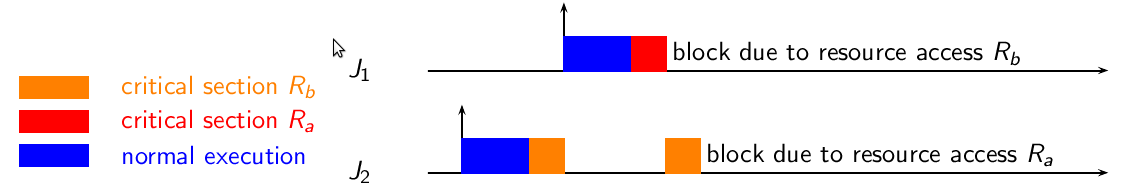
\includegraphics[width=0.9\textwidth]{PIP-deadlock}

  \end{itemize}
  
  However, if the resource accesses for a task are \blue{properly
    nested}, then some analysis is still possible.
  \begin{itemize}
  \item all the required semaphores are locked at once, or
  \item only one semaphore is used to guard one critical section, or
  \item a critical section guarded by a semaphore is \blue{completely} within another
    critical section guarded by another semaphore with a predefined
    access order, or
  \item \red{other ways} to prevent deadlocks. 
  \end{itemize}
\end{frame}

\begin{frame}
  \frametitle{Other ways? Priority Ceiling Protocol (PCP)}

  \begin{itemize}
  \item \underline{\textcolor{red}{Two key assumptions}}:
    \begin{itemize}
    \item The assigned priorities of all jobs are fixed.
    \item The resources required by all jobs are known a priori before
      the execution of any job begins.
    \end{itemize}
  \item Definition: The \emphblue{priority ceiling} of a resource $R$ is the 
    highest priority of all the jobs that require $R$, and is denoted 
    $\Pi(R)$. 
  \item Definition: The \emphblue{current priority} of a job $J$ at
    time $t$ is denoted 
    $\pi(t, J)$, initialized to the jobs priority level when $J$ is
    released. (smaller means higher priority) 
  \item Definition: The \emphblue{current priority ceiling} $\Pi'(t)$ of the
    system is equal to the highest priority ceiling of the resources
    currently in use at time $t$, or $\Omega$ if no resources are
    currently in use. $\Omega$ is a priority lower than any real
    priority.
  \item Use the priority ceiling to decide whether a higher priority
    can allocate a resource or not.
  \end{itemize}  
\end{frame}


\begin{frame}
  \frametitle{Theoretical PCP}
  \footnotesize
  \begin{enumerate}\small
  \item Scheduling Rule
    \begin{itemize}
    \item Every job $J$ is scheduled based on the
      current priority $\pi(t, J)$.
    \end{itemize}
  \item Allocation Rule: Whenever a job $J$ requests a resource R at
    time $t$, one of the following two conditions occurs:
    \begin{itemize}
    \item $R$ is held by another job and $J$ becomes blocked.
    \item $R$ is free:
      \begin{itemize}
      \item If $J$'s priority $\pi(t, J)$ is higher than the current
        priority ceiling $\Pi'(t)$, $R$ is allocated to $J$.
      \item Otherwise, only if $J$ is the job holding the resource(s)
        whose priority ceiling equals $\Pi'(t)$, $R$ is allocated to
        $J$
      \item Otherwise, $J$ becomes blocked.
      \end{itemize}
    \end{itemize}
  \item Priority-inheritance Rule: When $J$ becomes blocked, the job
    $J_l$ that blocks $J$ inherits the current priority $\pi(t, J)$ of J.
    $J_l$ executes at its inherited priority until it releases every
    resource whose priority ceiling is $\geq \pi(t, J)$ (or until it
    inherits an even higher priority); at that time, the priority of
    $J_l$ returns to its priority $\pi(t', J_l)$ at the time $t'$ when it was
    granted the resources.
  \end{enumerate}
\end{frame}

\begin{frame}
\frametitle{Exercises (10 points)}
\begin{enumerate}
\item Please activate PIP for DOUBLE\_SEMAPHORE example and see whether it does work. Draw the diagram. (3 points)
\item Please complete the code of PCP to get rid of the deadlock due to the resource competition. (7 points)
\end{enumerate}
\begin{columns}
    \column{\textwidth}
  \begin{table}
    \centering
    \begin{tabular}{|c|c|c|c|c|c|}
      \hline
     Tasks & Period & Critical Section & Arrive Time & Semaphore\\
     \hline
     $\tau_1$ & $20$ & $6$ & $2$ & II\\
     \hline
     $\tau_2$ & $30$ & $0$ & $5$ & X\\
     \hline
     $\tau_3$ & $40$ & $6$ & $0$ & I\\
     \hline
    \end{tabular}
  \end{table}
    %\column{0.35\textwidth}
  \end{columns}
\end{frame}

\end{document}
